\section{Proof of Concept}
Seguono una serie di screenshot della versione corrente realizzata ai fini dello studio di fattibilità del progetto.
\paragraph*{Topologia di esempio}
Si propone la seguente topologia di rete con alcuni test di connettività:
\newline\\
\begin{figure}[h!]
    \centering
    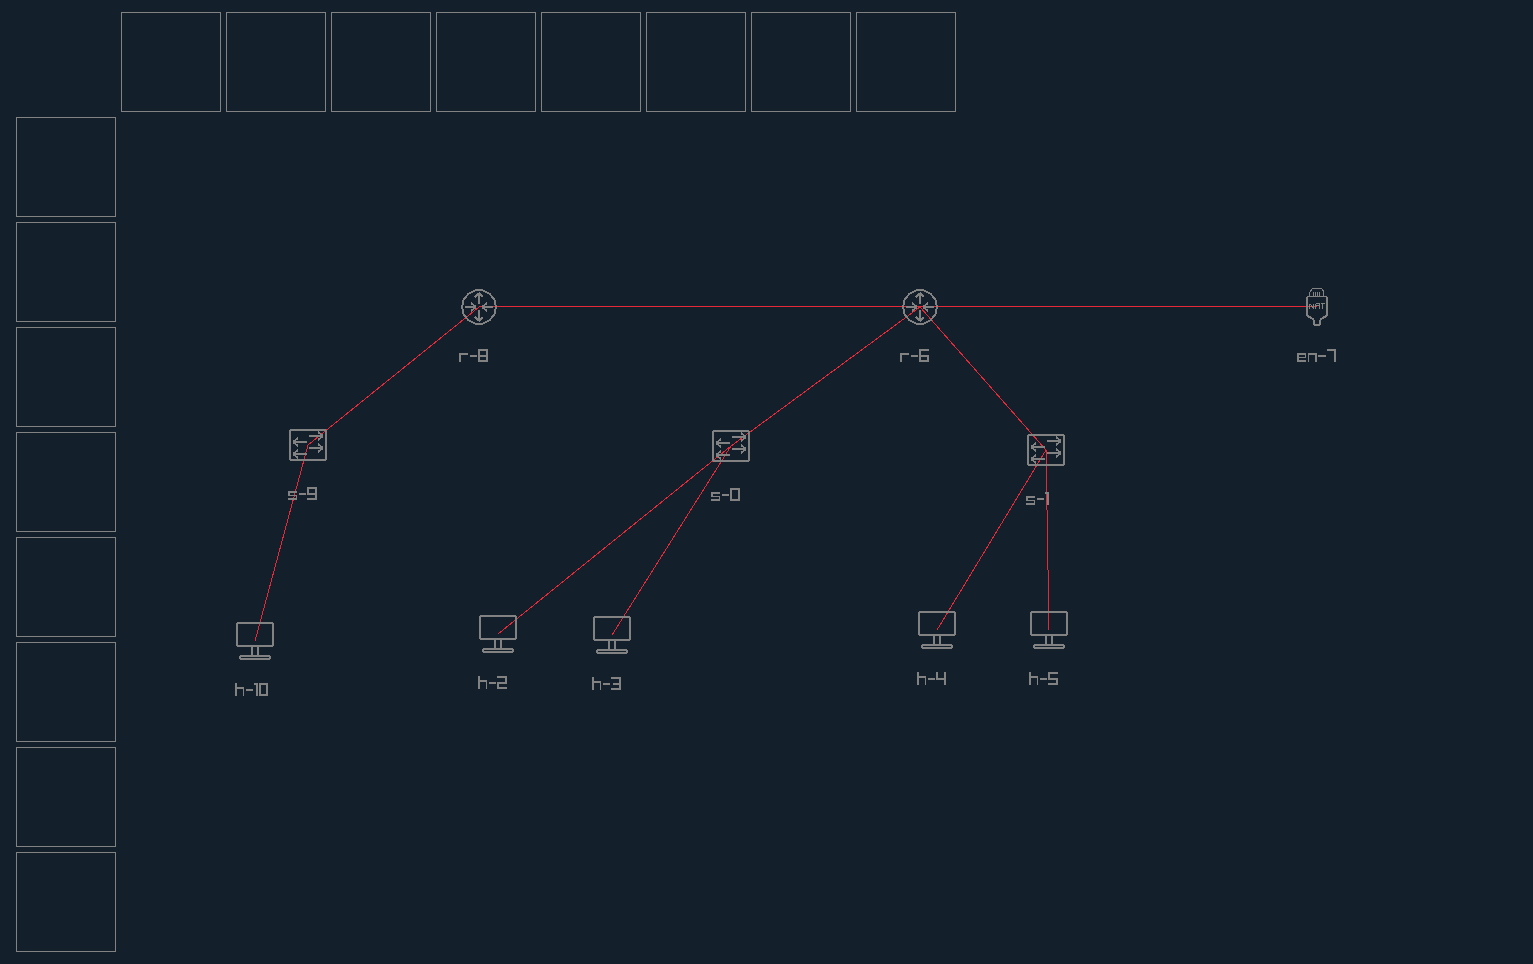
\includegraphics[width=14cm]{../images/poc_1.png}
    \caption[short]{Alcune subnet collegate ad un'interfaccia esterna con NAT.}
\end{figure}
\begin{figure}[h!]
    \centering
    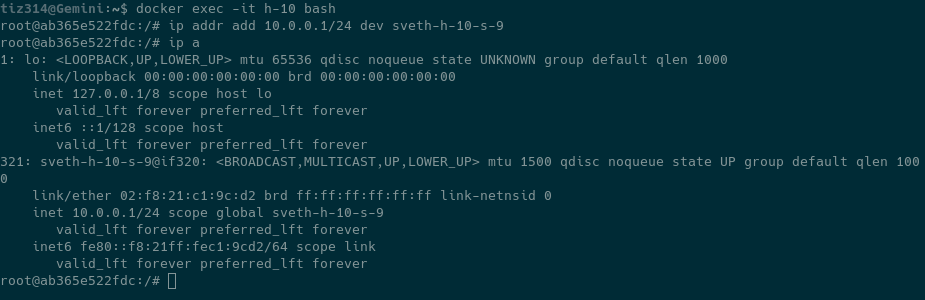
\includegraphics[width=14cm]{../images/poc_2.png}
    \caption[short]{Assegnamento IP ad \texttt{h-10}.}
\end{figure}
\pagebreak
\begin{figure}[h!]
    \centering
    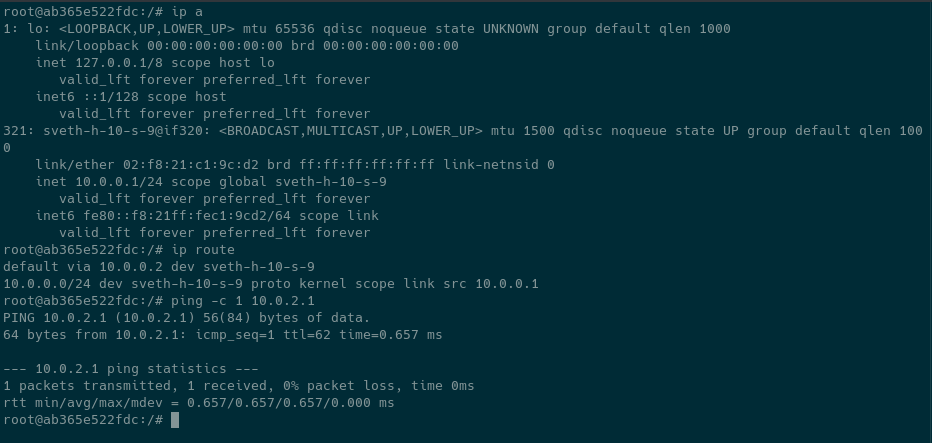
\includegraphics[width=14cm]{../images/poc_3.png}
    \caption[short]{Ping tra \texttt{h-10} ed \texttt{h-2}.}
\end{figure}
\begin{figure}[h!]
    \centering
    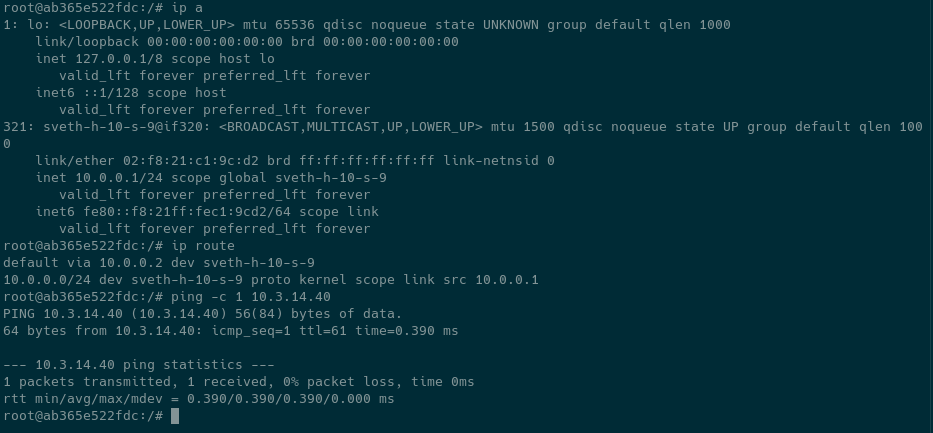
\includegraphics[width=14cm]{../images/poc_4.png}
    \caption[short]{Ping tra \texttt{h-10} e host fisico.}
\end{figure}
\paragraph*{Sviluppi futuri}
Tra gli sviluppi futuri prevediamo:
\begin{itemize}
    \item Interfaccia grafica migliorata e più \textit{user-friendly};
    \item Connessione con CLI direttamente da DONE;
    \item Salvataggio delle topologie.
\end{itemize}




\newpage